% ============================================================
% AdMIRe 2.0 System Description Paper
% YZV405E Group 100 — Hazar Utku Sözer, Faruk Rıza Öz, Enis Furkan Kırmızı
%
% Compile:
%   1. Download the ACL 2023 style files from https://github.com/acl-org/acl-style-files
%      and place acl.sty, acl_natbib.bst in this directory.
%   2. pdflatex report && bibtex report && pdflatex report && pdflatex report
% ============================================================

\documentclass[11pt]{article}
\usepackage{acl}  % non-anonymous, no line numbers (course submission, not blind review)
\usepackage{times}
\usepackage{latexsym}
\usepackage{microtype}
\usepackage{inconsolata}
\usepackage{booktabs}
\usepackage{amsmath}
\usepackage{graphicx}
\usepackage{tikz}
\usepackage{url}
\usetikzlibrary{arrows.meta, positioning, shapes.geometric}

% ============================================================

\title{Caption-Centric Idiom Ranking: A Frozen-Encoder Pipeline\\
       for AdMIRe 2.0 Subtask A}

\author{
  Hazar Utku Sözer \quad Faruk Rıza Öz \quad Enis Furkan Kırmızı \\
  Department of Artificial Intelligence and Data Engineering \\
  Istanbul Technical University \\
  \texttt{\{sozer20, ozf20, kirmizie23\}@itu.edu.tr}
}

\begin{document}
\maketitle

% ============================================================
\begin{abstract}
We describe our system for AdMIRe 2.0 Subtask A, where the goal is to rank five
candidate images by how well each captures the meaning of a possibly-idiomatic
nominal compound in a context sentence. We chain three off-the-shelf models
without fine-tuning any of them: NLLB-200 translates each sentence into English,
Phi-3.5-mini rewrites it by replacing the compound with its plain meaning, and a
logistic regression classifier on BGE-M3 embeddings decides whether to use the
paraphrase or the original sentence as the ranking query. Images are then ranked
by cosine similarity between the BGE-M3 embedding of that query and each image's
English caption. The classifier reaches 94.1\% accuracy (80/85) on the English
dev set, and the full pipeline scores 0.37 Top-1 accuracy on the Codabench
leaderboard, averaged across all 15 languages, which is +0.07 over a vanilla
SigLIP2 baseline. We then ran six rounds of ablations swapping out each
component, and none of them moved the top score. We argue this is because image
captions describe what's literally in the picture, not what it symbolizes, so
text-to-caption matching cannot bridge the gap between a figurative query and a
figuratively-intended image.
\end{abstract}

% ============================================================
\section{Introduction}

Nominal compounds (NCs) such as \textit{bad apple} or \textit{armchair general}
often mean something completely different from what their individual words
suggest \cite{nunberg1994idioms,sag2002multiword}. Figuring out whether a
speaker means the literal or the idiomatic reading from context is a core
problem in figurative language processing \cite{tayyarmadabushi2022semeval}.
AdMIRe 2.0 \cite{admire2026} pushes this problem into the visual world: given
a sentence with a potentially idiomatic NC, the system has to rank five
candidate images by how well each one matches the intended meaning.

What makes the task hard is that the images are deliberately tricky. The
``strongly figurative'' image illustrates the idiomatic meaning through a
concrete, literal scene, while the ``strongly literal'' image just shows the
words of the compound. Picking the right one requires both reading the idiom
correctly and reasoning about how an abstract idea can be drawn as a picture.
Vision--language models (VLMs) trained on regular image--caption pairs aren't
great at either of these in combination
\cite{yuksekgonul2023aro,thrush2022winoground}.

Given the time and compute we had, we went for a practical setup: instead of
fine-tuning anything, we wired together three frozen models and added a small
classifier we could actually train on the EN and PT-BR data. The idea we kept
coming back to is that every image already comes with an English caption, so we
can turn the problem from image--text matching into text--text matching. BGE-M3
\cite{chen2024bge} is a strong multilingual text encoder, so aligning a
paraphrased query with these captions is more reliable across 15 languages than
asking SigLIP2 to align the original sentence with each image directly.

Our contributions are: (1) a training-free ranking pipeline that scores 0.37
Top-1 accuracy on Codabench across all 15 languages (+0.07 over vanilla
SigLIP2); (2) a calibrated logistic regression classifier that picks idiomatic
vs.\ literal usage with 94.1\% accuracy (80/85) on English dev; and (3) a
six-round ablation study showing that the 0.37 score sits at a hard ceiling
that swapping individual components doesn't break.

% ============================================================
\section{Related Work}

\paragraph{Figurative language and multimodal grounding.}
Idiomatic expressions have been studied in computational linguistics for
decades \cite{nunberg1994idioms,sag2002multiword}. SemEval-2022 Task 2
\cite{tayyarmadabushi2022semeval} released a multilingual idiomaticity
detection benchmark in English and Brazilian Portuguese, and we lean on the
same kind of supervision (EN + PT-BR) for our classifier. AdMIRe 1.0
\cite{semeval2025admire1} was the first version of the image-ranking task at
SemEval-2025; the top system (PALI-NLP) hit 0.93 Top-1. AdMIRe 2.0 raises the
difficulty quite a lot: 15 languages, updated annotation rules, and a more
careful figurative--literal image set.

\paragraph{Concurrent AdMIRe 2.0 systems.}
Several teams have published system descriptions for the same shared task.
\citet{hosseinikivanani2026polyframe} freezes CLIP-style and BGE-M3 encoders
and trains only lightweight modules on top -- idiom-aware paraphrasing, an
LR-based sentence-type predictor, and Borda rank fusion -- with paraphrasing
identified as the main contributor. \citet{cotiga2026dcsn} bridges literal
and figurative meaning by generating auxiliary text (an idiomatic-meaning
explanation plus a literal visual description) and then voting with an
ensemble of CLIP models. The auxiliary-text idea is closest to our paraphrase
step, but they apply it on the image side via CLIP while we apply it on the
query side via BGE-M3. \citet{site2026itunlp} and \citet{umut2026itunlp2},
both from our own department, instead pursue zero-shot LLM-based pipelines.
Our design differs from all of these in dropping image embeddings from the
main path and relying on caption matching gated by a small learned
classifier.

\paragraph{Vision-language models.}
CLIP \cite{radford2021clip} popularised contrastive image--text pretraining.
SigLIP \cite{zhai2023siglip} swapped the InfoNCE loss for a sigmoid one and
improved zero-shot classification, and SigLIP2 \cite{siglip2_2025} added
stronger multilingual transfer and higher-resolution encoders (we use
\texttt{google/siglip2-so400m-patch16-512}). BLIP-2 \cite{li2023blip2} added a
small querying transformer between a frozen visual encoder and a language
model. The catch is that these models behave like bag-of-words on tasks that
need compositional or relational understanding
\cite{yuksekgonul2023aro,thrush2022winoground}, which is one reason we
fall back on text-to-caption matching instead of trusting image embeddings
directly.

\paragraph{Multilingual text encoders.}
BGE-M3 \cite{chen2024bge} produces 1024-dimensional embeddings and works well
across 100+ languages out of the box. We use it twice: once to embed the
paraphrased sentence for the classifier, and once to score similarity between
the query and each image caption. For translation we use the 600M distilled
NLLB-200 \cite{nllb2022} so everything runs locally on the GPU without hitting
any external API.

\paragraph{Lightweight paraphrasing.}
Phi-3.5-mini-instruct \cite{phi3_2024} is a 3.8B-parameter instruction model
that fits in our 12\,GB GPU at 4-bit (about 2.5\,GB VRAM). We use it to
rewrite each translated sentence so that the NC is swapped for a plain-English
description of its meaning. The rewritten sentence is what the ranker actually
matches against captions.

% ============================================================
\section{Task and Dataset}

Each instance in AdMIRe 2.0 Subtask A is a context sentence with a target NC
plus five candidate images. The images come from five fixed categories:
strongly figurative (SF), mildly figurative (MF), mildly literal (ML),
strongly literal (SL), and distractor (D). For idiomatic sentences the gold
ranking is SF$>$MF$>$ML$>$SL$>$D; for literal sentences it flips to
SL$>$ML$>$MF$>$SF$>$D. The catch is that the system isn't told whether the
sentence is idiomatic or literal at test time, so it has to figure that out
from context.

Only English and Brazilian Portuguese have labeled training data (506
instances together); the other 13 languages are zero-shot. The full test set
has 2{,}663 instances over 749 unique NCs and 4{,}845 images, each with an
auto-generated English caption. All sentences with the same NC share the same
five images; what changes between idiomatic and literal sentences is just the
expected ranking.

The main metric is Top-1 accuracy (does the top-ranked image match gold
position 1), averaged across all 15 languages. NDCG@5 with weights
$[3,1,0,0,0]$ is a secondary tiebreaker.

% ============================================================
\section{System Description}

Our pipeline, illustrated in Figure~\ref{fig:pipeline}, processes each instance
in three sequential steps.

\begin{figure}[t]
\centering
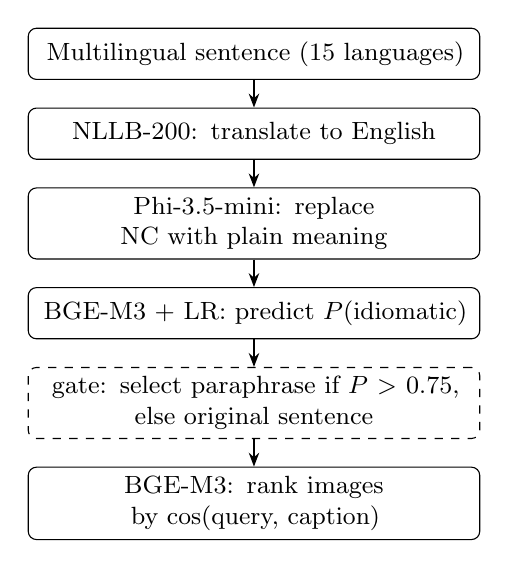
\begin{tikzpicture}[
    node distance=0.35cm,
    box/.style={rectangle, draw, rounded corners=3pt,
                text width=5.5cm, align=center,
                minimum height=0.65cm, font=\small},
    sbox/.style={rectangle, draw, rounded corners=3pt, dashed,
                text width=5.5cm, align=center,
                minimum height=0.65cm, font=\small},
    arr/.style={-{Stealth[length=5pt]}, thick}
]
  \node[box]  (sent) {Multilingual sentence (15 languages)};
  \node[box, below=of sent]  (nllb) {NLLB-200: translate to English};
  \node[box, below=of nllb]  (phi)  {Phi-3.5-mini: replace NC with plain meaning};
  \node[box, below=of phi]   (clf)  {BGE-M3 + LR: predict $P(\text{idiomatic})$};
  \node[sbox, below=of clf]  (gate) {gate: select paraphrase if $P > 0.75$,\\
                                     else original sentence};
  \node[box, below=of gate]  (rank) {BGE-M3: rank images by $\cos(\text{query, caption})$};

  \draw[arr] (sent) -- (nllb);
  \draw[arr] (nllb) -- (phi);
  \draw[arr] (phi)  -- (clf);
  \draw[arr] (clf)  -- (gate);
  \draw[arr] (gate) -- (rank);
\end{tikzpicture}
\caption{Pipeline overview. Dashed box marks the classifier gate; all encoders
         are frozen throughout.}
\label{fig:pipeline}
\end{figure}

\paragraph{Step 1: Translation.}
We translate every non-English, non-Portuguese sentence into English with
\texttt{facebook/nllb-200-distilled-600M} \cite{nllb2022}. EN and PT-BR
sentences pass through unchanged. Translations are cached as a Parquet file,
so we only pay the inference cost once.

\paragraph{Step 2: Paraphrasing.}
\texttt{microsoft/Phi-3.5-mini-instruct} \cite{phi3_2024} (4-bit, $\approx$2.5
GB VRAM) rewrites each translated sentence so the NC is replaced by a plain
description of its meaning. For example, given \textit{bad apple} in an
idiomatic context, we get a sentence about one person whose bad behavior drags
down a larger group. The paraphrase is meant to spell out what the speaker
actually meant, so the ranker doesn't have to guess from the surface form.

\paragraph{Step 3: Sense classification and ranking.}
We train a logistic regression classifier with isotonic calibration (5-fold
CV) on BGE-M3 embeddings of the paraphrased EN and PT-BR training sentences.
At inference it outputs a calibrated $P(\textit{idiomatic}) \in [0,1]$ per
instance, which we use to pick the ranking query:

\begin{equation*}
  q = \begin{cases}
    \text{paraphrase} & P(\textit{idiomatic}) > 0.75 \\
    \text{translated sentence} & \text{otherwise}
  \end{cases}
\end{equation*}

Images are then ranked by cosine similarity between the BGE-M3 embedding of
$q$ and the BGE-M3 embedding of each image's English caption.

\paragraph{Why this design.}
SigLIP2's text encoder was trained on short literal English captions paired
with images, so it tends to do worse on idiomatic phrasing and on
machine-translated non-English text. The auto-generated captions, on the
other hand, are exactly the kind of short literal English BGE-M3 was trained
on. So pushing everything through captions and using a strong multilingual
text encoder gave us a cleaner signal than trying to align sentences with
images directly.

% ============================================================
\section{Experiments and Results}

\paragraph{Baselines.}
We use two SigLIP2 baselines: \textit{orig\_only}, plain image--text cosine
similarity with no paraphrase or classifier (0.28), and \textit{classifier\_a0.3},
the Category-Aware Heuristic Ranker from our project proposal that applies an
$\alpha$-penalty over visual features (0.30). The latter was our originally
proposed final ranker; the ablations below show why we replaced it with the
simpler caption-matching gate.

\paragraph{Ablation protocol.}
We ran six rounds of ablations, each one changing a single design choice while
keeping the rest fixed. All scores below are Top-1 accuracy on the Codabench
blind test set, averaged across the 15 languages.

\begin{table}[t]
\centering
\small
\begin{tabular}{llc}
\toprule
\textbf{Round} & \textbf{Configuration} & \textbf{Top-1} \\
\midrule
Baselines
  & \textit{orig\_only} (SigLIP2, no classifier)         & 0.28 \\
  & \textit{classifier\_a0.3} (SigLIP2 + heuristic)      & 0.30 \\
\midrule
R1: Signal
  & BGE-M3 caption, always paraphrase                    & 0.35 \\
  & \textbf{BGE-M3 caption, classifier-gated}            & \textbf{0.37} \\
  & SigLIP2 (30\%) + BGE-M3 (70\%) ensemble              & 0.37 \\
\midrule
R2: Paraphraser
  & Qwen2.5-7B-Instruct, classifier-gated                & 0.37 \\
\midrule
R3: Similarity
  & BGE-reranker-v2-m3 (cross-encoder)                   & 0.35 \\
\midrule
R4: Pipeline
  & PT-BR via NLLB + soft blend                          & 0.36 \\
\midrule
R5: Threshold
  & Sweep 0.50--0.85 (best)                              & 0.37 \\
\midrule
R6: Enrichment
  & Enriched captions only                               & 0.33 \\
  & Enriched + original blend                            & 0.34 \\
  & 3-way: orig + enriched + SigLIP2                     & 0.36 \\
\bottomrule
\end{tabular}
\caption{Top-1 accuracy for all submitted configurations.
         Bold marks our best submission.}
\label{tab:results}
\end{table}

\paragraph{Round 1 -- Ranking signal.}
The biggest single jump (+0.07) comes from switching the ranker from SigLIP2
image--text alignment to BGE-M3 caption matching. Adding the classifier gate
on top is worth another +0.02, because it sends literal sentences back to the
original text instead of forcing them through the paraphrase. Mixing SigLIP2
back in as an ensemble doesn't help, which suggests the visual signal isn't
adding anything that wasn't already in the caption.

\paragraph{Round 2 -- Paraphraser quality.}
Swapping Phi-3.5-mini for Qwen2.5-7B-Instruct (much bigger, stronger
instruction-following) gives the exact same 0.37. So the paraphraser isn't
what's holding us back.

\paragraph{Round 3 -- Similarity model.}
BGE-reranker-v2-m3 \cite{bge_reranker} is a cross-encoder, which usually beats bi-encoders on
text relevance, but here it only scored 0.35. We read that as a signal that
the difficulty in this task isn't really about ranking text similarity more
precisely.

\paragraph{Round 4 -- Pipeline changes.}
Routing PT-BR through NLLB before paraphrasing actually hurt (0.36). Phi-3.5
handles Portuguese directly better than it handles Portuguese-translated-to-
English. A soft probability-weighted blend (instead of the hard gate) also
didn't help.

\paragraph{Round 5 -- Threshold sweep.}
Top-1 stays flat at 0.37 for any threshold $\geq 0.60$ and only drops to 0.36
below that, where the gate gets too eager and routes too many literal
sentences through the paraphrase. The 0.75 default we shipped with is fine.

\paragraph{Round 6 -- Caption enrichment.}
We tried having Phi-3.5 append an extra sentence to each caption explaining
what abstract concept the image might symbolize. We expected this to help,
but it was the worst result in the whole study: pure enriched captions
dropped to 0.33, blending the original back in recovered to 0.34, and adding
SigLIP2 as a third channel only got us back to 0.36. Every variant of
enrichment we tried made things worse.

% ============================================================
\section{Analysis}

\paragraph{The visual metaphor gap.}
All six rounds basically point at the same thing. The ``strongly figurative''
image for \textit{bad apple} is probably something like people sitting around
a meeting table -- it shows the consequence of one bad person, not the rotten
fruit and not the abstract idea of corruption. The caption then describes a
meeting, which is technically accurate but doesn't say anything about the
idiomatic meaning. Our query (the paraphrase) talks about that idiomatic
meaning. So no matter how good the paraphrase or the encoder is, we're trying
to match two things that don't share vocabulary. This is the same kind of
problem \citet{yuksekgonul2023aro} identified for VLMs, just shifted
into the caption--text setting.

\paragraph{Why cross-encoders didn't help.}
Cross-encoders normally beat bi-encoders at picking up fine-grained text
similarity, so it was a bit surprising that BGE-reranker-v2-m3 underperformed.
The way we read it is that the bottleneck isn't that the bi-encoder is too
coarse -- it's that the caption simply doesn't contain the information the
query is asking about, and a more expressive matcher can't recover information
that isn't there.

\paragraph{Role of the classifier.}
The logistic regression classifier gets 94.1\% accuracy (80/85, precision
0.935, recall 0.956) on the English dev set and is worth +0.02 over always
running the paraphrase path. It generalises to the zero-shot languages because
BGE-M3 puts paraphrases of idiomatic sentences in roughly the same region of
embedding space across languages. We can't push the gain further than +0.02
though, because the ceiling is set by the caption-matching step, not by how
accurate the classifier is.

\paragraph{Comparison to AdMIRe 1.0.}
PALI-NLP scored 0.93 Top-1 on AdMIRe 1.0 \cite{semeval2025admire1}, close to
the 0.83 human ceiling. Our 0.37 suggests AdMIRe 2.0 is much harder, or at
least that frozen off-the-shelf models don't get you very far on this version
of the task. To get closer to human performance you probably need to actually
train end-to-end on figurative--literal image rankings.

% ============================================================
\section{Conclusion}

We built a modular pipeline of three frozen models for AdMIRe 2.0 Subtask A
that scores 0.37 Top-1 across 15 languages. The main takeaway is that BGE-M3
caption matching is a much cleaner signal than SigLIP2 image--text alignment
(+0.07). Six rounds of ablations later, the score is still 0.37: changing the
paraphraser, the similarity model, the classifier threshold, the translation
path, and even the caption content didn't move the top number. We think the
ceiling comes from the gap between what a figurative query is asking and what
an image caption literally says.

Two directions seem worth trying next. First, contrastive fine-tuning on the
EN and PT-BR gold rankings to learn a small projection layer that aligns
figurative queries with figurative images directly, instead of going through
captions at all. Second, asking a VLM to re-caption each image in terms of
what it symbolizes rather than what it shows -- more expensive, but it would
attack the gap from the caption side instead of the query side.

% ============================================================
\section*{AI Usage Statement}
As required by the course, we disclose how we used AI tools. Phi-3.5-mini-instruct
is part of the system itself: we used it to paraphrase all 2{,}663 test
instances by replacing each NC with a plain-English description of its meaning.
Outside the system, we used Claude (claude-sonnet-4-6, Anthropic) as a coding
assistant during implementation and for structural feedback while writing this
report. Experimental design, analysis, and conclusions were ours. A running
log of every AI-assisted session, with prompts and decisions, is maintained
in the project repository at
\url{https://github.com/hazarsozer/YZV405E_2526_100/blob/main/AI_USAGE.md}.

% ============================================================
\bibliographystyle{acl_natbib}
\bibliography{references}

\end{document}
